\chapter{AI and Medicine}

Marc Andreessen has famously claimed that software will eat the world \cite{andreessen2011software}.  Andrej Karpathy has argued that AI will eat software \cite{karpathy2017software}.  It follows then that AI will eat the world.  It has already begun to eat many problems in medicine.

An early example of AI applied to medicine is the work of Professor Daphne Koller and her lab in 2011 \cite{beck2011systematic}.  They applied probabilistic graphical models (before the neural net boom) to detect breast cancer in histology slides.  Their work showed that researchers in the AI lab with technical backgrounds outside of medicine could make contributions to medicine -- a field often thought of as a walled garden.  

In 2015 Bharath Ramsundar in Professor Vijay Pande's group showed that deep learning could be applied to drug discovery \cite{ramsundar2015massively}.  They first created a dataset of 40 million measurements across more than 200 biological targets from public sources.  They showed that, with further refinements, deep learning could be used for virtual drug screening.  Traditionally the process takes many years of research.

In 2016, Lily Peng and others demonstrated results in detecting diabetic retinopathy from images taken with retinal cameras \cite{gulshan2016development}.  Diabetic retinopathy is the fastest growing cause of blindness, with over 400 million diabetic patients worldwide.  If caught early, it can be treated.  Otherwise it leads to irreversible blindness.  Traditionally, diabetic eye disease is detected when a specialist examines pictures of the back of the eye and rates them for disease presence and severity. Severity is determined by the type of lesions present, for example microaneurysms, hemorrhages, or hard exudates.  These indicate bleeding and fluid leakage in the eye.  She worked with doctors in India and the US to create a dataset of 128,000 images, each of which was evaluated by 3 to 7 ophthalmologists from a panel of 54 ophthalmologists.  Verily has since deployed this technology in India for population screening.

This large dataset of retinal images was further leveraged to assess cardiovascular risk factors \cite{poplin2018prediction}.  They found they could distinguish smokers from nonsmokers 71\% of the time.  They could predict blood pressure to within 11 mmHg, on par with a traditional blood pressure cuff.  These results show the value of collecting a large labeled medical dataset.

In 2017, it was shown that skin cancer could be detected in pathology slides \cite{liu2017detecting}.  This is interesting because these pathology slides show skin at the cellular level, which is the reasonable level of abstraction to visually observe dividing cancer cells.  An issue for humans reading pathology slides is that there are so many cells to look at that they can easily miss obvious signs of cancer.  Fortunately computers do not get bored and are pretty quick.  The researchers showed that they could scan 10 gigapixel histology slides of skin cells digitized at 40x magnification and outperform a pathologist (89\% vs 73\% FROC score).  This work was further refined in 2019 to create ``Microscope 2.0" \cite{chen2019augmented}.

It was then shown that deep learning could assist pathologists with better results than replacing them \cite{steiner2018impact}.  That is, assisted pathologists achieved higher accuracy than either the algorithm or the pathologist alone. Algorithm assistance significantly increased the sensitivity of detection for micrometastases from 83\% to 91\%. Average review time per image also decreased with assistance from 116 seconds to 61 seconds.

In late 2018, researchers at Google took this work further and applied it to detecting prostate cancer \cite{nagpal2019development}.  They collected a dataset of 112 million pathologist-annotated image patches from 1226 slides.  They trained a neural net on this data and compared performance with board-certified pathologists.  Compared to a reference standard provided by genitourinary pathology experts, the mean accuracy among 29 general pathologists was 61\% on the validation set. Google achieved 70\%, beating the board-certified pathologists.

In 2020, researchers at Google used images of skin lesions along with metadata such as age, gender, and other information to diagnose skin conditions \cite{liu2020deep}.  Their dataset included 16,114 cases collected from a teledermatology practice serving 17 sites.  They trained a neural net to distinguish between 26 different skin conditions which comprise 80\% of the cases seen in primary care.  They compared top-1 accuracy with dermatologists, primary care physicians, and nurse practitioners.  Their net scored 66\%, dermatologists scored 63\%, primary care physicians scored 44\%, and nurse practitioners scored 40\%.  This showed that primary care physicians and nurse practitioners could use a neural net to detect skin conditions as well as dermatologists can.

Healthcare data is in the process of becoming more digitized.  There is no common data representation across vendors, each uses a different way to structure their data.  Also, sites that use the same vendor may differ significantly.  For example, they typically use different codes for the same medication. Further, data can be spread over many tables, some containing encounters, some containing lab results, and yet others containing vital signs. The Fast Healthcare Interoperability Resources (FHIR) standard addresses many of these challenges \cite{mandel2016smart}. It has a solid extensible data-model, is built on established web standards, and is quickly becoming the standard for individual records and bulk-data access.  

In 2018, a collaboration between Google, UC San Francisco, Stanford Medicine, and University of Chicago was able to build a deep learning model on electronic health records using the FHIR protocol \cite{rajkomar2018scalable}.  The dataset contained data collected from over 200,000 patients hospitalized for at least 24 hours.  They achieve 0.94 AUC at predicting in-hospital mortality, 0.75 AUC at predicting 30-day unplanned readmission, 0.86 AUC at predicting a prolonged length of stay, and 0.9 AUC at predicting all of the patient's discharge diagnoses.

Later work published in 2020 showed that using the FHIR records, a deep learning system could be trained that predicts what medications a physician might prescribe given the patient's medical history \cite{rough2020predicting}.  They gathered a dataset of 3 million medication orders from over 100 thousand hospitalizations.  93\% top-10 lists contained at least one medication that would be ordered by clinicians for the given patient within the next day.  This suggests a deep learning system could be used to recommend medication orders to physicians.

In 2019, it was shown that deep learning could perform on par with radiologists at detecting 4 different conditions in X-rays \cite{majkowska2020chest}.  They gathered a dataset of 870 thousand labeled X-ray images.  Their net achieved 0.95 AUC for detecting ``pneumothorax", 0.72 AUC for ``nodule or mass", 0.91 AUC for ``airspace opacity", and 0.86 AUC for ``fracture".

Recently DeepMind showed significant progress in the elusive field of protein folding \cite{senior2020improved}.  From a raw genetic sequence of As, Ts, Cs, and Gs, AlphaFold can correctly predict the resulting protein structure on par with experimental procedures.  In fact it even predicted the correct structure of a particular protein that had been eluding researchers for 10 years.  The next phase of evolution will either be AI or genetic engineering. 

A major obstacle that AI and medicine has faced is the lack of large datasets openly available to researchers.  In fact this is the dilemma neural nets in general faced until about 2012.  Neural nets have been around since at least the 1980s when Yann Lecun automated hand written digit recognition of zip codes \cite{lecun1989backpropagation}.  The rule of thumb was always that neural nets were the 3rd best solution.  Convex solutions like SVM often worked better.  Why have these non-convex neural nets had a resurgence all of a sudden?  Many people credit it to Krizhevsky, dominating the image recognition challenge ILSVRC with AlexNet \cite{krizhevsky2012imagenet}.  I would credit it to Professor Fei-Fei Li and her group for creating ImageNet in the first place \cite{deng2009imagenet}.  Creating a large dataset was not considered a glamorous task.  Many researchers would rather invent a genius algorithm, not do the dirty work of creating a dataset.  But what we have seen again and again is that it is not about the algorithm.  Little has changed from the 80s algorithmically.  What has changed is the amount of compute available, and the size of dataset available.  Andrew Ng has a nice plot that shows the performance of a neural net as dataset increases \cite{ng2016nuts}.  More data, more parameters, better performance.  We are seeing this in NLP with GPT3 \cite{brown2020language}.  GPT3 is trained with a very simple algorithm.  Give it a sequence of text, minus one word, and train it to predict the missing word.  After training on 45 terabytes of internet text and consuming 314 zettaflops of compute, GPT3 can generate essays that are nearly indistinguishable from human.

That said, there are some improvements being made to the algorithms.  For example, residual layers added great value to convolutional neural nets \cite{he2016deep}.  Very deep highway networks with skip connections can be trained much more aggressively, overcoming the problem of vanishing gradients.  Recently, transformer networks have been outperforming both recurrent and convolutional neural nets at many tasks.  When I started grad school, the NLP and Computer Vision groups had little in common other than that they were both in the same building.  After the ImageNet breakthrough, and Andrew Ng's 700+ person machine learning courses, many research groups started to use deep learning.  At least then there was a common framework with which to make progress.  Things like stochastic gradient descent algorithms, or ideas like data augmentation, could be shared between domains.  Recently, we are even seeing the same type of neural net architecture being shared between domains.  So there is some value in improving the algorithms.  

But the most successful pursuits in AI are often by those who have the most data and compute.  NVIDIA has played a big role in making more compute available to researchers.  But it was only when Andrew Ng's grad students painstakingly wrote GPU kernels to train a neural net \cite{raina2009large} that NVIDIA became relevant in AI. And before ImageNet, no datasets were large enough to justify doing this.  Before ImageNet, researchers used hand-crafted features and then something like an SVM or random forests on top.  After ImageNet, the features could be learned from data.  Large ImageNet-like datasets are critical for making progress in AI and medicine.  When I undertook the skin cancer project, no such dataset existed.  The greatest hurdle was creating the large dataset of skin lesion images.  This is one of the reasons I have so much respect for ImageNet.  Because of the growing excitement about machine learning and AI, many large organizations are responding to the call to action.  The UK, for example, has created a dataset, UK Biobank, comprising over half a million people \cite{sudlow2015uk}.  The data collected includes everything there is know about a patient: MRI scans, full genome sequence, blood tests, diagnoses, demographics, and much more.  There are two similar projects in the US underway.  One is run by Verily called Project Baseline.  The other is run by the US government called All of Us.  Large medical datasets like this will be essential for future progress in AI and medicine.

A big issue in medicine in privacy.  Privacy is somewhat at odds with the requirements of AI.  AI usually requires a large centralized dataset, which means users have to send the data over the internet somewhere.  Google faces a similar problem with many of their products.  How can they train on user data without breaching their privacy?  To deal with this Google invented federated learning and it has been gaining popularity \cite{bonawitz2019towards}.  Essentially data stays on the user's device.  A parameter gradient is computed on-device and sent to the server to update the model.  Another approach is differential privacy \cite{abadi2016deep}.  This approach has nice theoretical properties but destroys a lot of the data.  Applying AI to medicine will require privacy respecting methods for data collection.

Another big issue with AI and medicine is regulation.  FDA approval can easily cost millions of dollars and require lengthy clinical trials.  This prevents the classic Silicon Valley approach of moving fast and breaking things.  And maybe startups should be prevented from breaking people in the process of trying to make them healthier.  This dilemma has a lot in common with that of self driving cars.  How can automated driving get smarter without learning from mistakes?  Maybe some day, preventive healthcare algorithms and self driving car algorithms will have similar approaches.  Maybe some kind of safe reinforcement learning.

\section{Dermatology}
The first step in classifying skin lesions is to create a dataset.  There is no ImageNet of skin cancer.  There are, however, many dermatology websites with semi-labeled images that doctors upload.  I scraped all the images from one dermatology website and fine-tuned AlexNet on the 20 or so labels they were categorized into.  At the time, my dad happened to have a spot on his leg that he was concerned about.  The fine-tuned AlexNet said it was likely a benign seborrheic keratosis.  A dermatologist collaborator confirmed that it was in fact a benign seborrheic keratosis.

After that I scraped every single image I could find online of a skin lesion.  This started by simply searching different keywords.  With these searches, quite a few repositories turned up where doctors were uploading images of skin lesions along with the diagnoses.  Each website had its own unique pattern with how it presented images and labels.  A python script was written for each website.  I continued website by website, custom python script by custom python script, scraping every single dermatology website I could find on the Internet.  Once all the images were scraped, some images were used for a reverse image search.  New repositories turned up.  These websites were all in other languages. The English keywords had been missing them.  After scraping these foreign websites, with foreign language labels, the raw dataset doubled in size.

After months of scraping, I had a messy set of 300k images, many of which were not even pictures of skin lesions, and whose diagnosis labels were in many different languages.  The labels varied from site to site.  Sometimes it was the caption of the image.  Sometimes it was the title of the page.  Further, the labels were high entropy strings.  For example ``malignant melanoma" and ``melanoma, malignant" are two different strings with the same meaning.  A list of categories is required to train a classifier with.  The length of the set of labels, i.e. the number of categories, was chosen as the metric for how ``clean" the label set was.  The size of the set should be as small as possible, but no smaller.  A few simple heuristics helped significantly. All the labels were converted to ASCII lowercase and stripped of excess white space.  All foreign labels were translated to English. A similarity matrix between all pairs of strings was computed using Levenshtein distance.  The highest scoring matches were merged.  Many simple heuristics that did not require any medical knowledge were applied.  Then with a significantly reduced set of labels, the dermatologists helped organize further.  A blank file was created for every disease label and put into one big folder.  The dermatologists created more folders and subfolders and placed the disease files into them.  Using only Windows File Explorer, they created a taxonomy of the scraped labels.

The images also needed to be cleaned up.  There were many images of skin cells under a microscope.  50 microscope images and 50 skin images were fed into an AlexNet to train a binary classifier.  The net learned to distinguish microscope vs skin images with minimal validation loss in only a few iterations.  It was let loose on the entire dataset to filter out the microscope images.  A similar filtering procedure was applied to images that were not skin lesions.  This time, a random set of images from ImageNet were used as the not-skin category.

Now the dataset was significantly cleaned and contained over 129k images and about 2,000 diseases, 2 orders of magnitude larger than any previously used dataset.  By this point, Google had open sourced Inception v3 \cite{szegedy2016rethinking} -- an upgrade from AlexNet \cite{krizhevsky2012imagenet} and lighter weight than VGG \cite{simonyan2014very}.  Inception was fine tuned with this gigantic dataset.  The results were great, too good in fact.  Upon closer inspection, there were problems in the dataset.  The train/test partition was contaminated with duplicates.  This manifested itself in two ways.  First, the same image sometimes showed up on multiple websites and second, there were often multiple images of the same lesions taken from slightly different angles and distances.  See Figure \ref{fig:derm_data_problems}.  Further some of the images had color coated stickers or other giveaway markers on them that made the diagnosis easier.

\begin{figure}
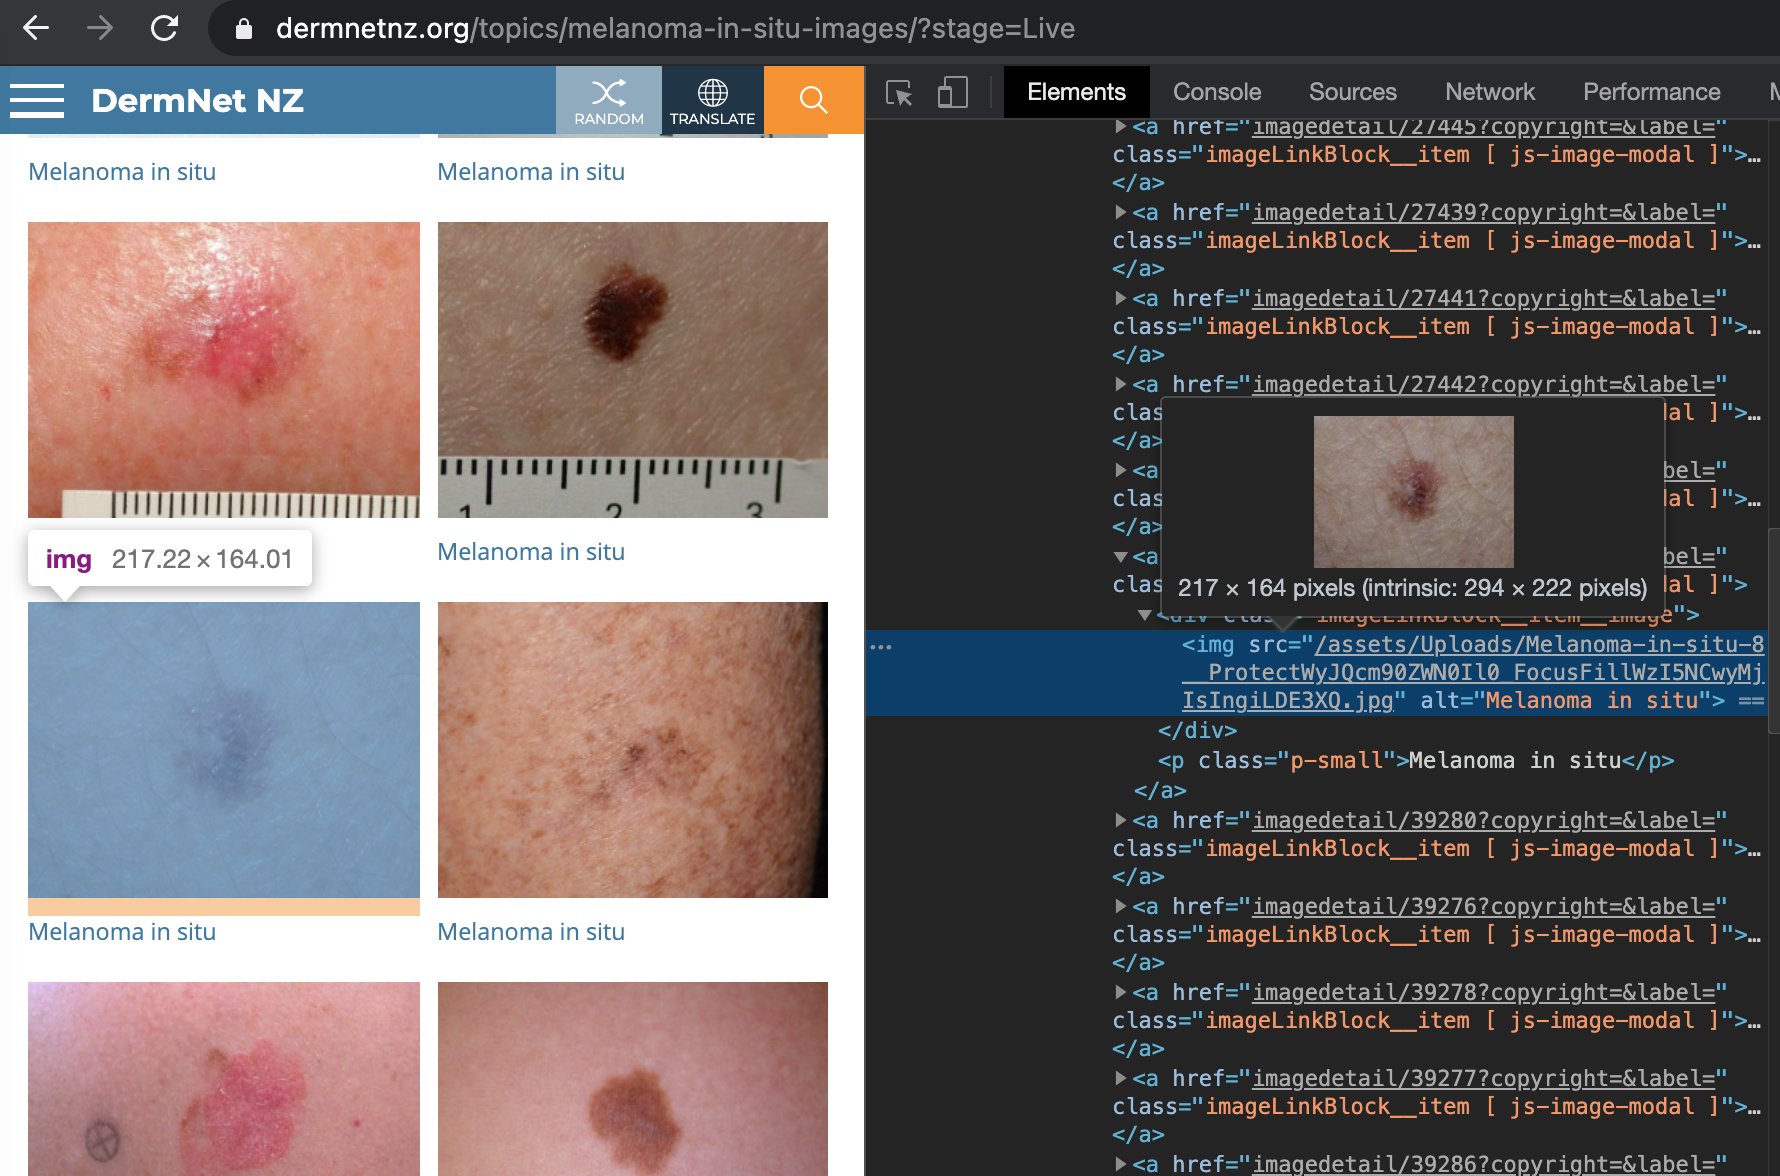
\includegraphics[width=\textwidth]{derm_scrape}
\caption{Data Collection}
\vspace{12px}
Collecting the data involved many ad-hoc python scripts to extract the image and label.  An example of an image URL and its raw label embedded in HTML is shown here.
\label{fig:derm_scrape}
\end{figure}

\begin{figure}
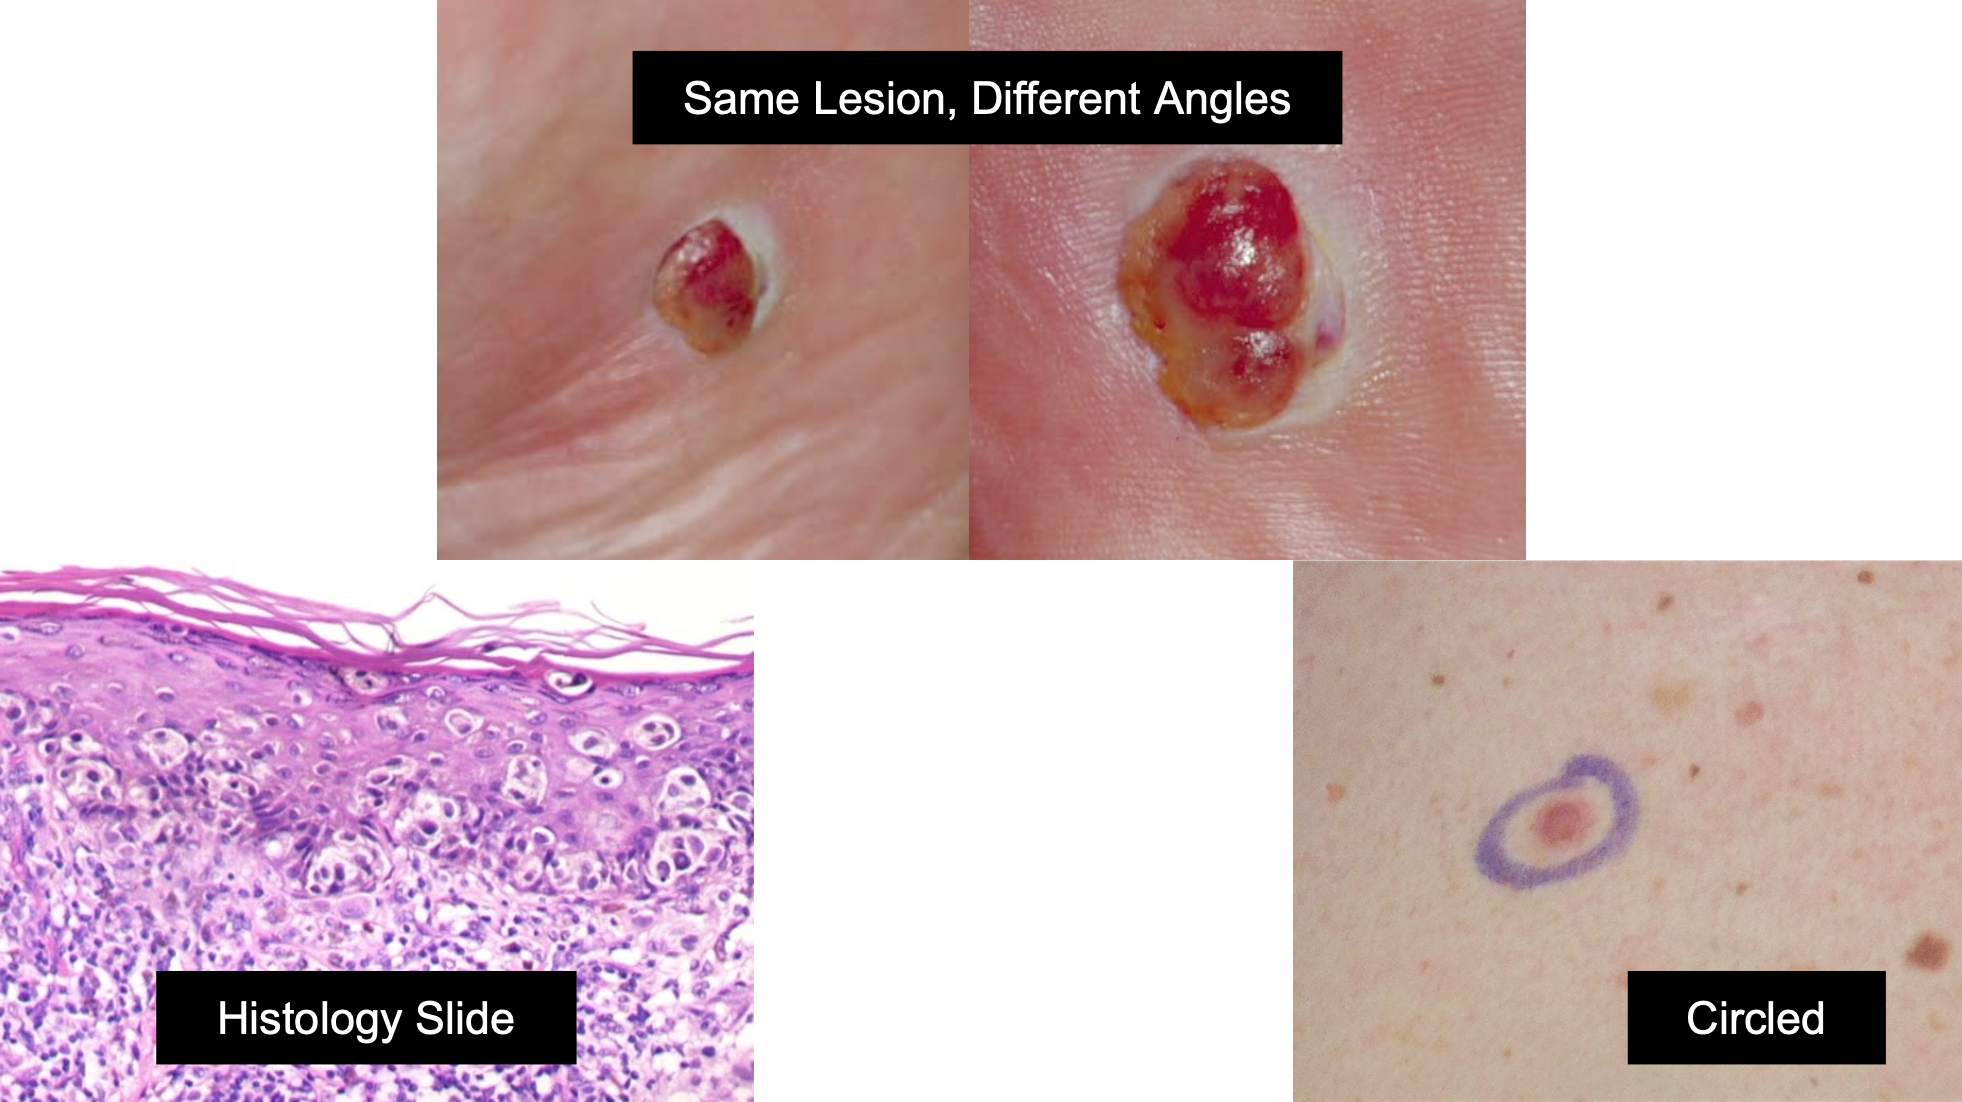
\includegraphics[width=\textwidth]{derm_data_problems}
\caption{Data Problems}
\vspace{12px}
The data had to be dealt with carefully.  Images of histology slides were filtered out.  Multiple images of the same lesion from different angles could not be split across training and validation datasets.  Giveaways such as circles and stickers could not be used for validation.
\label{fig:derm_data_problems}
\end{figure}


These issues were dealt with in a few different ways.  First, the image metadata often contained information on when the photo was taken.  A simple heuristic of not separating images taken within an hour apart helped significantly.  The problem however was that not all of the images contained the EXIF metadata.  Amazon Turk was then used to detect duplicates.  To deal with the giveaway markers, those images were only used for training, not testing.  These heuristics helped to partition the data into fair training, validation, and testing datasets.

But there were still problems.  The diagnoses were not necessarily biopsy proven.  Any doctor could upload an image to some of these sites with their diagnosis without any biopsy proof.  A biopsy proven diagnosis involves cutting a piece of the lesion off, slicing it, and analyzing it under a microscope.  This requires a highly trained dermatopathologist.  To have a truly clean test set, biopsy proven images were required and they needed to be fully disjoint from the training and validation datasets.  To achieve this two reliable sources of biopsy proven skin lesion images were used.  The first source was Stanford hospital.  A training course was required just to get access to Epic -- the database Stanford uses to save data.  The second source was a for-purchase set of images from the UK that all had biopsy proven diagnoses.  With those two sources a pristine test set could now be set aside.

Since the diseases were laid out in a tree there were some options as to how to train the net.  In one extreme skin lesions could be simply classified as benign or malignant where any disease with malignant as its ancestor was malignant and all other diseases were benign.  But this throws away the fine-grained information.  The other extreme is to train on every single disease.  The problem with this approach is that many of the diseases had only a few images.  So the net had very little chance at learning that fine grained label through the fine-tuning procedure.  A compromise was made to use the finest grain classification possible with the constraint that each node contained at least 1000 images.  At inference time the probability the net assigns to malignant is computed as the sum of the probabilities assigned to its descendants.

To evaluate the performance of the net at detecting malignant skin cancer, sensitivity and specificity are computed.  This allows direct comparison of performance with dermatologists.  In the clinic, a dermatologist is faced with the decision of whether to biopsy a lesion or to not biopsy it.  If they choose to biopsy the lesion, a dermatopathologist will slice it up and view the individual cells under a microscope.  This results in a near-perfect diagnosis.  Sensitivity is defined as the number of true positives divided by the number of positives.  For a dermatologist in the clinic, that is the number of malignant lesions they choose to biopsy divided by the number of malignant lesions they see.  Similarly, specificity is calculated as the number of benign lesions they do not biopsy divided by the number of benign lesions they see.

\begin{figure}
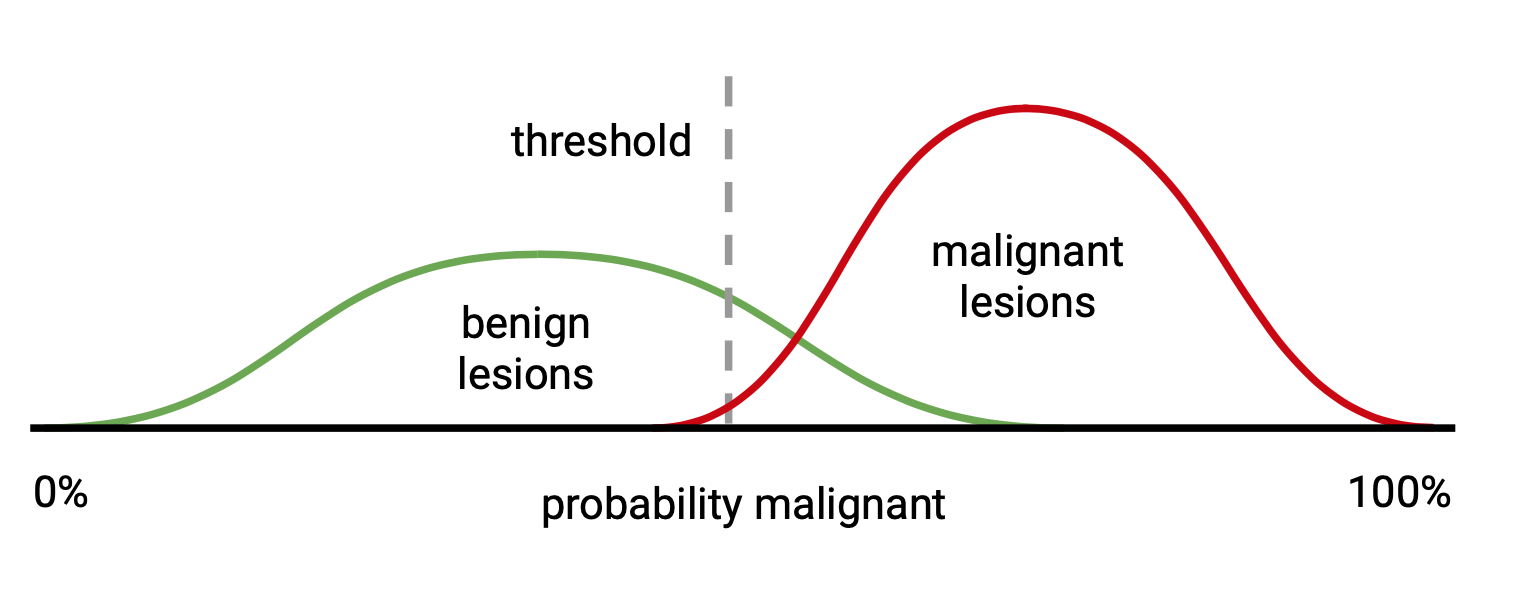
\includegraphics[width=\textwidth]{derm_sens_class}
\caption{Example Sensitive Classifier}
\vspace{12px}
When evaluating a skin lesion it is important to err on the side of predicting that it is malignant if it is benign than the predict that it is benign if it is malignant.  That is, false negatives are more dangerous than false positives.  In the case of a false positive, the lesion is simple biopsied, little harm done.  In the case of a false negative, the patient leaves thinking they are healthy but actually has cancer that may have been easily treatable.  To make a prediction the net must either classify the lesion as benign or malignant, not output a probability.  Therefore there needs to be a probability threshold with which any probability above it is malignant and anything below it is benign.  Consider the conditional distributions of net probabilities given whether the lesion is benign or malignant shown above.  The threshold is chosen such that almost all malignant lesions lie above the threshold, resulting in very few false negatives.  This threshold corresponds to a sensitive classifier.
\vspace{12px}
\label{fig:derm_sens_class}
\end{figure}

For the network sensitivity and specificity are calculated a little bit differently.  The network outputs probabilities that are added up the tree to obtain the probability of being malignant.  Based on this probability a decision must be made of whether to classify the lesion as malignant or benign.  Only then can the net be evaluated as scoring a true positive, a true negative, a false positive, or a false negative, and from there sensitivity and specificity over the entire test set be computed.  See Figure \ref{fig:derm_sens_class} for an example of a sensitive classifier.  With a sensitive classifier, almost every malignant lesion is detected.  The cost of a sensitive classifier is usually that there are more false positives and the specificity is lower.  In the case of biopsying a lesion, it is better to err on the side of cutting off a lesion that is benign than to miss a malignant melanoma.

By varying the threshold, all possible sensitivity and specificity pairs can be computed, effectively not making a decision on what the threshold should be.  This is done for 3 binary classification tasks.  The first task is picking apart basal cell carcinomas from their benign lookalikes.  Basal cell carcinoma is the most common form of skin cancer.  The second task is picking apart melanomas from their benign lookalikes.  Melanoma is the most deadly form of skin cancer.  The third task is again picking apart melanomas from their benign lookalikes, but this time with dermoscopy images.  Dermoscopy images are photos taken with a special device called a dermoscope that shines polarized light and captures information just beneath the skin.

A group of 25 dermatologists were tested from Stanford, University of Pennsylvania, University of Iowa, and Massachusetts General Hospital with images of malignant and benign lookalike skin lesions.  They were shown an image and asked whether they would biopsy the lesion or not.  Then a sensitivity and specificity could be computed for each dermatologist.  The network was evaluated on the same images, sweeping the threshold to calculate all sensitivity specificity pairs.  For most of the dermatologists there is some threshold for which the net will simultaneously achieve both a higher sensitivity and a higher specificity.  It was concluded that dermatologist level performance was achieved.  It is important to note that this test does not fully capture what would happen in the clinic.  A dermatologist would be able to ask the patient questions, look at the lesion from different angles, and touch it.  Another thing to note is how surprisingly varied the dermatologists are in their performance.  Maybe humans should not be trusted with this task.  This will be explored further in Chapter 3.

% In all I scraped and organized over 100k images, creating the largest ever skin lesion image dataset known to AI.  It was during this time that I gained appreciation for ImageNet.  A lot of work went into creating this skin lesion dataset that a neural net could train on.  For example, the labels were high entropy strings.  The labels "malignant melanoma" and "melanoma, malignant" would be two totally different categories to a neural net.  The labels were streamlined with the help of simple heuristics and our dermatologist collaborators.  The dermatologists helped categorize all the high entropy string labels into a nice taxonomy of diseases.  This allowed for later choosing the granularity desired to train with.  A coarse granularity would be benign vs malignant.  One could traverse the taxonomy further to get finer grained categories.  If the categories are too fine, not many images will be available for a given category.  There is a happy medium somewhere between the coarse benign vs malignant, and something too fine grained like basal cell carcinoma on left forearm vs basal cell carcinoma on right forearm.  In the former case, one would have many images for each category.  In the latter case, there may be 1 or 2 images in each category.  Another issue that came up was that many photos weren't actually photos of skin lesions.  Some were histology slides, others were computer generated figures.  To deal with this, I grabbed 100 images of manually verified skin lesions.  Then I grabbed 100 images of all the things I didn't want in the dataset.  I finetuned AlexNet to do binary classification on skin vs not skin.  It achieved really good accuracy on a held out test set so I let it loose on all the data.

\section{Critical Care}

In some sense fine-tuning an image classifier was fairly straightforward because image classification is a highly studied topic and tons of research hours have gone into finding the optimal architecture and learning the most effective set of weights.  What other ubiquitous sensors can detect life threatening medical conditions? Here are a few examples of readily available consumer products:

\begin{itemize}
    \item Scales that measure bio-impedance across the body between left and right feet
    \item Fingertip PPG sensors that use infrared light to measure blood flow beneath the skin
    \item Infrared thermometers
    \item Blood pressure cuffs
    \item ECGs that measure voltage across the heart between the left and right pointer fingers
    \item Blood analyzers that measure glucose and ketones from a single drop of blood
    \item Metabolic blood panel, lipid blood panel, complete blood count
\end{itemize}

The PPG and ECG sensors were exciting because they were noninvasive and measured raw waveforms.  This data seemed amenable to a 1D ConvNet.  There is a metric called pulse transit time \cite{geddes1981pulse}.  The idea is to measure the time it takes for a pulse to traverse the body from the heart to the fingertip.  This can be measured with ECG and PPG combined.  Pulse transit time is an interesting metric because it is highly correlated with blood pressure.  If blood pressure is high, pulse transit time is low, and vice versa.  The issue is that it needs to be calibrated for each person to reliably measure blood pressure.  This is, in theory, a great application for deep learning.  Throw out the hand crafted features and let the neural net learn to measure blood pressure reliably without calibration from raw ECG and PPG data.  Then use this device along with a blood pressure cuff to test the neural net on real people.

As with the skin cancer project, the first step was to gather data.  It turns out hospitals collect tons of this kind of data.  They collect other waveforms too such as respiration, and multiple ECG leads.  Further, they collect blood pressure as a waveform.  A dataset of 7 terabytes of the waveforms was downloaded and prepared for fast training.  Later I discovered that the ECG and PPG waveforms were misaligned.  A disclaimer stated that the waveforms could be misaligned by up to 500ms. Pulse transit time is on the order of about 100ms so this misalignment completely destroyed that information.  But maybe there was still enough information present in the waveforms to measure blood pressure.  Net after net was trained, tuning hyperparameters, changing the architecture.  The nets were performing better and better.  They were learning something about the waveforms that related to blood pressure.

In an effort to boost blood pressure performance, more labels were fed to the net: it was asked to predict age and gender, for example.  These additional training signals improved blood pressure estimation so more labels were added.  Every hospital admission was labeled with various ICD diagnosis codes.  The International Classification of Diseases, or ICD for short, is a taxonomy of all medical conditions, and is maintained by the World Health Organization.  This meant a new taxonomy did not need to be created from scratch as was done for the skin cancer work.  A taxonomy already existed.  The net was fed 90 different ICD diagnosis codes to learn.  It was still not very good at measuring blood pressure, but it was learning a lot about the ICD codes.  As a result, the focus was shifted to predicting these.  Here are a few of them:

\begin{itemize}
    \item Cardiogenic shock occurs when the heart cannot pump enough blood and oxygen to the brain, kidneys, and other vital organs.  It is often fatal if not treated immediately.  About half of patients survive if treated immediately.
    \item Systolic heart failure is when the left ventricle of the heart can’t contract completely.  The heart will not pump forcefully enough to move blood throughout the body in an efficient way
    \item A cerebral aneurysm is a weakness in the wall of a cerebral artery or vein that causes a ballooning of the blood vessel.  A ruptured aneurysm can cause serious health problems such as hemorrhagic stroke, brain damage, coma, and death.
    \item A myocardial infarction, also known as a heart attack, usually occurs when a blood clot blocks blood flow to the heart.  Without blood, tissue loses oxygen and dies
    \item Liver cirrhosis is the irreversible scarring of the liver.  It is caused by alcohol abuse and other sources.  In advanced cases a liver transplant may be needed.
\end{itemize}

\begin{figure}
\begin{center}
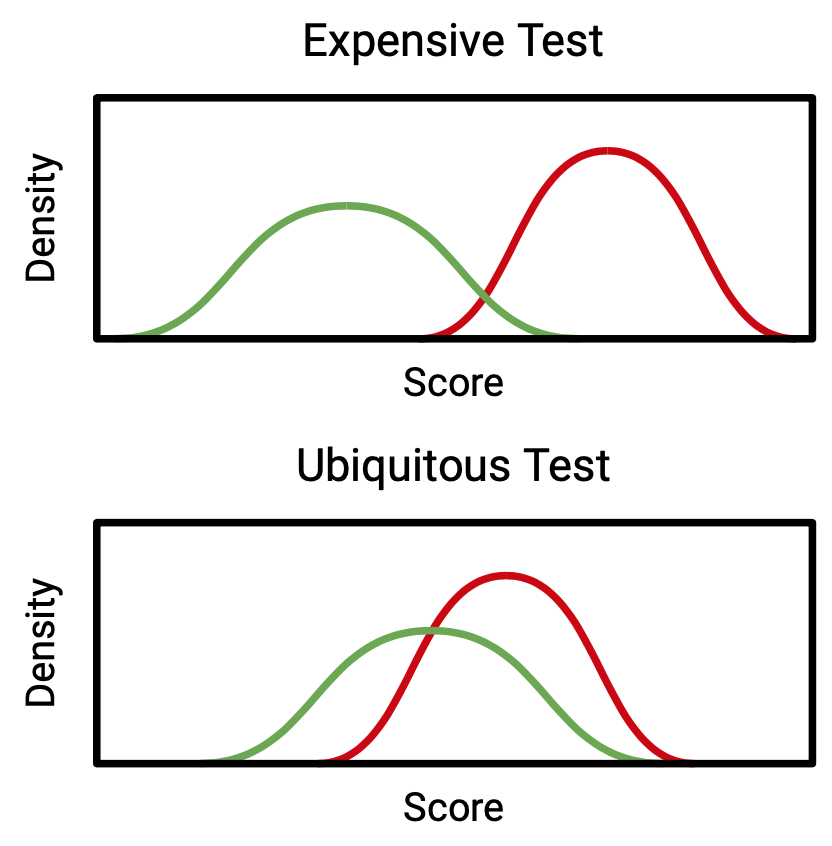
\includegraphics[width=0.8\textwidth]{icu_expens_ubiqu}
\end{center}
\caption{Effective Sensitivity Motivation}
\vspace{12px}
Can a cheap, ubiquitous, and maybe unreliable test be used to recommend patients for an expensive, limited, but more reliable test?  Consider the example conditional distributions shown above for 2 different classifiers, one expensive and one ubiquitous.  Green and red curves represent distributions over scores the net outputs given that the label is negative or positive, respectively.  The ubiquitous classifier does a poor job at separating the distributions of positive and negative cases, but still provides some information.  The score from the ubiquitous test can be used to triage users for the expensive test, increasing the expensive test's effective sensitivity.
\label{fig:icu_expens_ubiqu}
\end{figure}

So what can be done to detect these conditions with ubiquitous measurements?   Consider the example shown in in Figure \ref{fig:icu_expens_ubiqu}.  Imagine there is an expensive test for some condition that does pretty well at picking apart positive and negative cases.  This test is very expensive though and is not widely available.  

An MRI machine, for example, is a highly capable noninvasive imaging machine, and unlike X-rays and CT scans, does not harm the user with cancer causing radiation.  It can map the internals of the body in high detail and detect many medical conditions.  MRI machines are liquid helium cooled, superconducting technology marvels and cost millions of dollars.  A technician is required to run the machine and a radiologist to interpret the results.  It is really expensive and only available to people with suspected problems or people who are willing to pay a few thousand dollars for a scan.

On the other hand, imagine there is a ubiquitous test that is not as great at picking apart positive and negative cases.  It is not obvious what to do with the results of this test.  Setting a threshold anywhere results in a lot of false negatives and/or false positives. But it still provides some information.  How can that information be harnessed? 

About 1 in 5 Americans use a smartwatch or fitness tracker.  The Apple Watch is capable of measuring both a photoplethysmogram, aka PPG, and a lead I electrocardiogram, aka ECG.

A ubiquitous test can be used to improve the utility of an expensive test.  One could argue that an expensive unavailable test such as an MRI results in an enormous amount of effective false negatives for all the people who could have been diagnosed had they received the test, but due to a lack of availability were never tested.  Therefore the expensive test has a low effective sensitivity.  The ubiquitous test can improve the number of true positives detected by the expensive test if it is used for triage.  That is, if the highest scores on the ubiquitous test are funneled into the expensive test, the effective sensitivity of the expensive test will increase.  This will be further explored in Chapter 4.

% I took a radically different approach for task of detecting problems in waveform data.  I created a dataset from scratch once and wasn't trying to do that again.  This time I found a nice dataset collected by highly motivated grad students at MIT.  They collected raw data from many different sources within a Harvard teaching hospital.  Further, not only was the data collected, the labels were already in a taxonomy.  The labels were ICD codes, used for billing.  These ICD codes are part of a taxonomy that contains all known diseases.  So I didn't have to create the dataset and I didn't have to create the taxonomy.  But for this project, there wasn't an ImageNet pretrained model like VGG or Inception that I could use.  I had to invent my own model architecture.  For one, the signals were 1 dimension instead of 2 dimensions as are images.  Also, there wasn't a strong precedent on how to train a neural net on biological waveforms.  For images, it is common practice to train on resolutions of about 256x256.  What length input should one use for waveforms, though?  Ultimately I settled on 2048 sample inputs, or about 16 seconds.

% In this thesis I show results in applying AI to preventive healthcare in two domains.  The first domain is detecting skin cancer in images of skin lesions.  It is remarkable that harvesting raw internet images made it possible to achieve dermatologist level performance at classifying skin lesions.  If the raw data on the internet can be harnessed to match dermatologist performance, what other gold is waiting to be mined?  For one, there is GPT3. 

% The second domain is in assessing risk for various conditions from biological waveforms measured in the hospital such as ECG and PPG.  Here it is remarkable that from such simple waveforms, a neural net is able to develop a sense of what organ isn't working properly.  For example, the neural net knows when something is wrong with the brain.  This is evident in the semantic inference heat map.  When a patient has a condition affecting their brain, ICD codes that affect the brain will carry high risk.  Similarly, if a patient has a condition affecting their liver, ICD codes that affect the liver will carry high risk.  This is remarkable because maybe predicting the exact ICD code isn't what is important.  A given ICD code has many synonyms, and it is semi random which one a doctor will choose.  Maybe assessing organ health is the thing that is actually tangible.
